  \documentclass[14pt, oneside]{book}
    \usepackage[margin=1in]{geometry} 
    \usepackage[brazilian]{babel}
    \usepackage{graphicx}
    \usepackage[utf8]{inputenc}
    \usepackage[T1]{fontenc}
    \usepackage{amsmath,amsthm,amssymb,amsfonts}
    \usepackage{enumitem, verbatim}
    \usepackage{multicol}
    \usepackage{mathtools}
    \usepackage{titlesec}
    \usepackage{hyperref, color}
    \usepackage{float}
        \hypersetup{
            colorlinks=false, %set true if you want colored links
            linktoc=all,     %set to all if you want both sections and subsections linked
            linkcolor=blue,  %choose some color if you want links to stand out
        }
    \usepackage{listings}
    \titleformat{\chapter}[hang]{\bf\huge}{\thechapter}{2pc}{}
    \DeclarePairedDelimiter{\ceil}{\lceil}{\rceil}
    \date{\vspace{-5ex}}
    \lstset{language=Python}  
    \usepackage{pythonhighlight}
     
    \newcommand{\N}{\mathbb{N}}
    \newcommand{\Z}{\mathbb{Z}}
    \newcommand\tab[1][1cm]{\hspace*{#1}}
    \renewcommand{\qedsymbol}{$\blacksquare$}
     
    
\theoremstyle{definition}
    \newtheorem{problem}{Problema}
    \newtheorem{dica}{Dica}
    \newtheorem{gabarito}{Gabarito}
    \newtheorem{defn}{Definição}
    \newtheorem{teorema}{Teorema}
    
\begin{document}
    \pagenumbering{gobble}

    \begin{titlepage}
        \centering 
        
\includegraphics[scale = 0.8]{ufpe.png} \\
        \Large{\textbf{UNIVERSIDADE FEDERAL DE PERNAMBUCO}}\\
        \large{Departamento de Eletrônica e Sistemas}
        \vspace*{\stretch{2.0}}
   
        \Huge\textbf{ELETRÔNICA DIGITAL}\\
        \Large\textbf{DESPERTADOR/RELÓGIO/CRONÔMETRO}
   
        \vspace*{\stretch{2.0}}
        \vfill
        \Large{Arthur Santos Pimentel} \\
        \Large{Matheus Henrique Camilo de Araújo} \\
        \Large{Matheus Sobreira Farias} \\
        \Large{Pablo Godoy de Albuquerque}
        \\~\\
        \Large{Outubro, 2018}
    \end{titlepage}

\addtocontents{toc}{\protect\hypertarget{toc}{}}
\tableofcontents
\mainmatter
        \chapter[Motivação]{\hyperlink{toc}{Motivação}}
            \tab Como explicado no projeto anterior, existem linguagens de descrição de Hardware que podem descrever o funcionamento de um circuito e, portanto facilitar o trabalho do projetista ao sintetizar seu projeto em forma de circuito. Neste projeto, com o auxílio da linguagem de descrição AHDL, pode-se observar o avanço devido às ferramentas disponibilizadas por uma linguagem. A grande economia de tempo acarreta na produtividade e agilidade da implementação de um projeto. Por exemplo, quando a linguagem de blocos no último projeto foi usada, os grupos levaram em média duas semanas e meia para atingir as especificações do projeto. Agora, porém, com o auxílio de uma linguagem de descrição, nota-se que vários grupos concluiram o projeto mais cedo e tiveram tempo para debater as soluções de certos bugs. \\
	        \tab Ainda pode-se dizer que o uso de uma linguagem possibilitou a discussão sobre certos pontos do projeto entre integrantes do grupo, já que a descrição dos circuitos se tornou um processo menos mecânico. Quando os integrantes do grupo se dividiam em tarefas, geralmente, as ideias surgiam e os circuitos eram manualmente implementados no \textit{Quartus}. Agora, porém, os circuitos são interpretados pelo programa através de uma linguagem em códigos e transformadas nas versões mais simplistas de seus circuitos. Assim, o grupo se preocupa menos com a estética e a legibilidade do bloco e passa a focar em suas funcionalidades. \\
	        
           
            
        \chapter[Objetivos]{\hypertarget{obj}{}\hyperlink{toc}{Objetivos}}
             \tab Nesse projeto, foi utilizada a linguagem de descrição de Hardware AHDL, com o auxílio do software \textit{Quartus Prime 17.1} e da placa \textit{FPGA DE2-155}, ambos da \textit{Altera}, com o intuito de criar um relógio/despertador/cronômetro, seguindo os seguintes critérios:
            \begin{itemize}
                \item O sistema deve ser inicializado no modo relógio;
                \item O ajuste do despertador deve estar condicionado por uma chave;
                \item O ajuste do relógio ou despertador deve ser determinada por uma chave.
                \item Outra chave deve ser responsável por slecionar o modo cronômetro;
                \item Outra chave deverá selecionar qual alarme que deve ser selecionado (1 ou 2);
                \item Os botões da placa devem ser utilizados para efetuar o ajuste dos horários. Serão usados quatro botões para incrementar e decrementar as horas e os minutos.
                \item Serão utilizados quatro LEDs da placa para simular o acionamento do despertador.
            \end{itemize}
            
            
        \chapter[Implementação]{\hyperlink{toc}{Implementação}}
            \tab Para realizar a implementação do relógio, despertadores e cronômetro, foi utilizado o software \textit{Quartus Prime 17.1}, que é um software cuja função é ser um ambiente de desenvolvimento para linguagens de descrição de hardware, sendo assim, a placa a qual foi descrita pelo projeto foi a \textit{Altera DE2-115}. Foi utilizada ao longo do desenvolvimento a linguagem de descrição de hardware, AHDL. \\
            \tab Uma vez no software \textit{Quartus}, para facilitar a construção do projeto, foi decidido separá-lo em \textbf{5} módulos de desenvolvimento, dessa forma o grupo como um todo conseguiria agir paralelamente, para que o tempo fosse melhor otimizado, são estes os módulos: \textbf {Contador}, \textbf{Debounce}, \textbf{Comparador}, \textbf{Seleção de Operação} e \textbf{Indicador}.
            
            \section[Contador]{\hyperlink{toc}{Contador}}
                \tab Certamente o módulo mais importante de todo o projeto, o contador serve, como o próprio nome ja diz, para realizar a contagem do tempo. Para desenvolver o relógio/despertador/cronômetro, foi necessário separar os contadores de acordo com a necessidade.
                \subsection{Relógio}
                \tab No caso do relógio, foi utilizado $3$ contadores, sendo dois deles módulo $60$ (para os segundos e os minutos) e o último sendo módulo $24$ (para as horas), segue o código do contador dos minutos, o código do contador dos segundos e das horas possui logica análoga, nas Figuras \ref{fig:c1} e \ref{fig:c2}. \\
                \begin{figure}[H]
                    \centering
                    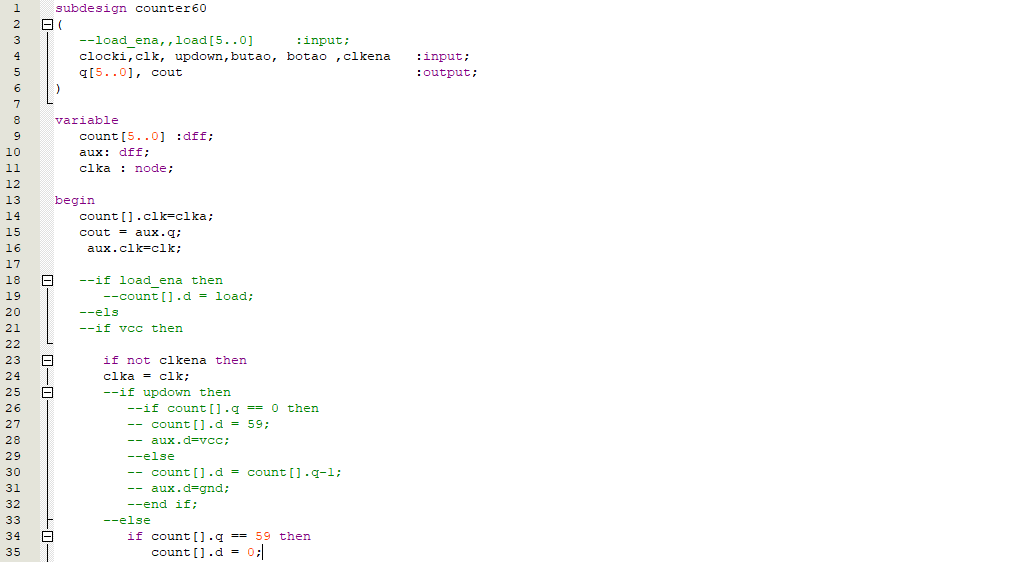
\includegraphics[scale=0.7]{cont60p1.png}
                    \caption{Código do Contador mod 60 Primeira Parte}
                    \label{fig:c1}
                \end{figure} \\
                
                \begin{figure}[H]
                    \centering
                    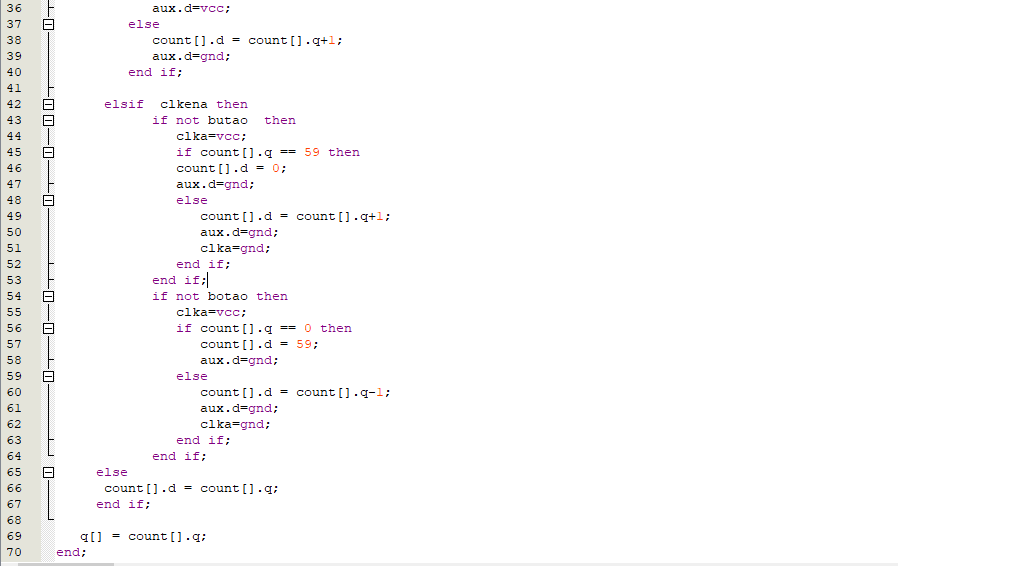
\includegraphics[scale=0.6]{cont60p2.png}
                    \caption{Código do Contador mod 60 Segunda Parte}
                    \label{fig:c2}
                \end{figure}\\
                
                \subsection{Despertadores}
                \tab Nos despertadores, não é interessante que apareça no display os segundos, dessa forma, para não ter que desenvolver outro codigo, foi utilizado o mesmo código do relógio, ou seja, foi implementado o despertador da mesma forma que o relógio, com os mesmos contadores, a diferença final é que ao passar pelo decodificado, os valores dos segundos foram apagados.
                \subsection{Cronômetro}
                \tab  Ao longo do desenvolvimento do projeto, foi necessário a implementação de um cronômetro que contasse segundos e minutos além de poder pausar e reiniciar. O cronômetro foi projetado a partir do modulo do contador de 60 segundos, partindo de seu código o cronômetro recebeu as duas novas funções, de \textit{pause} e \textit{reset}.\\
                
                \tab Obeserva-se na Figura \ref{fig:cronometro} a implementação do Módulo do Cronômetro.
                
                    \begin{figure}[H]
                    \centering
                    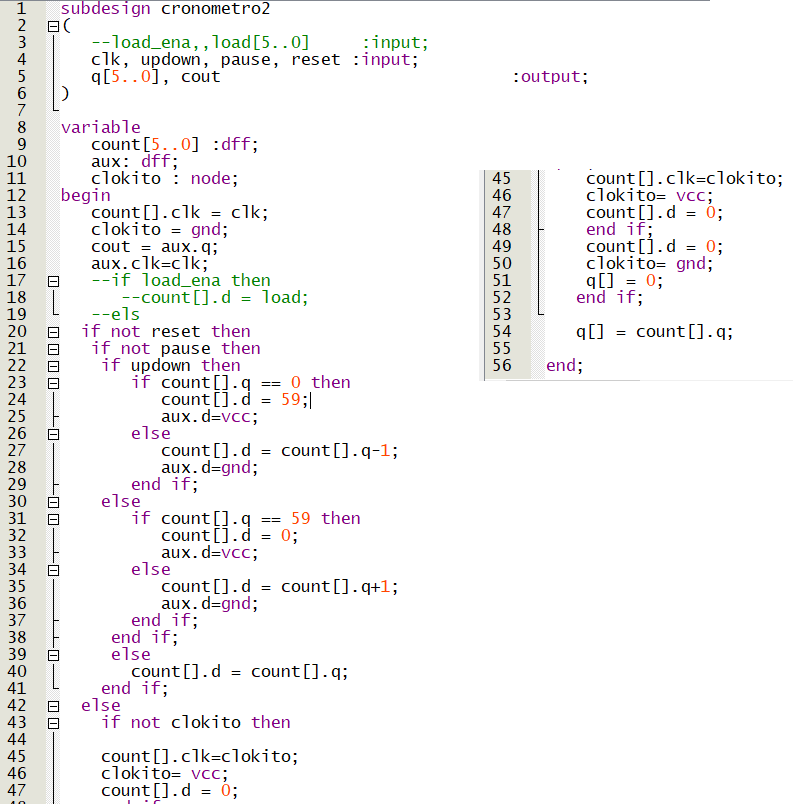
\includegraphics[scale=0.8]{cronometro2.png}
                    \caption{Cronômetro}
                    \label{fig:cronometro}
                \end{figure}
                
               
                
            \section[Módulo Debounce]{\hyperlink{toc}{Módulo Debounce}}
                \tab O módulo Debounce surgiu como necessário a partir de um problema que ocorreu durante uma tentativa de teste do grupo. Ao testar o projeto em diferentes placas do laboratório, ocorreu de uma delas estar com o botão desgastado, de forma que, pressionando o botão rapidamente várias vezes, o ajuste de hora não incrementava/decrementava corretamente, e para corrigir isso, precisou ser implementado tal módulo. \\
                \tab A ideia por trás do Debounce gira em torno do ruído que é causado pelo botão ou alavanca, durante o momento do pressionar, conforme segue na Figura \ref{fig:debounce2}. \\
                \begin{figure}[H]
                    \centering
                    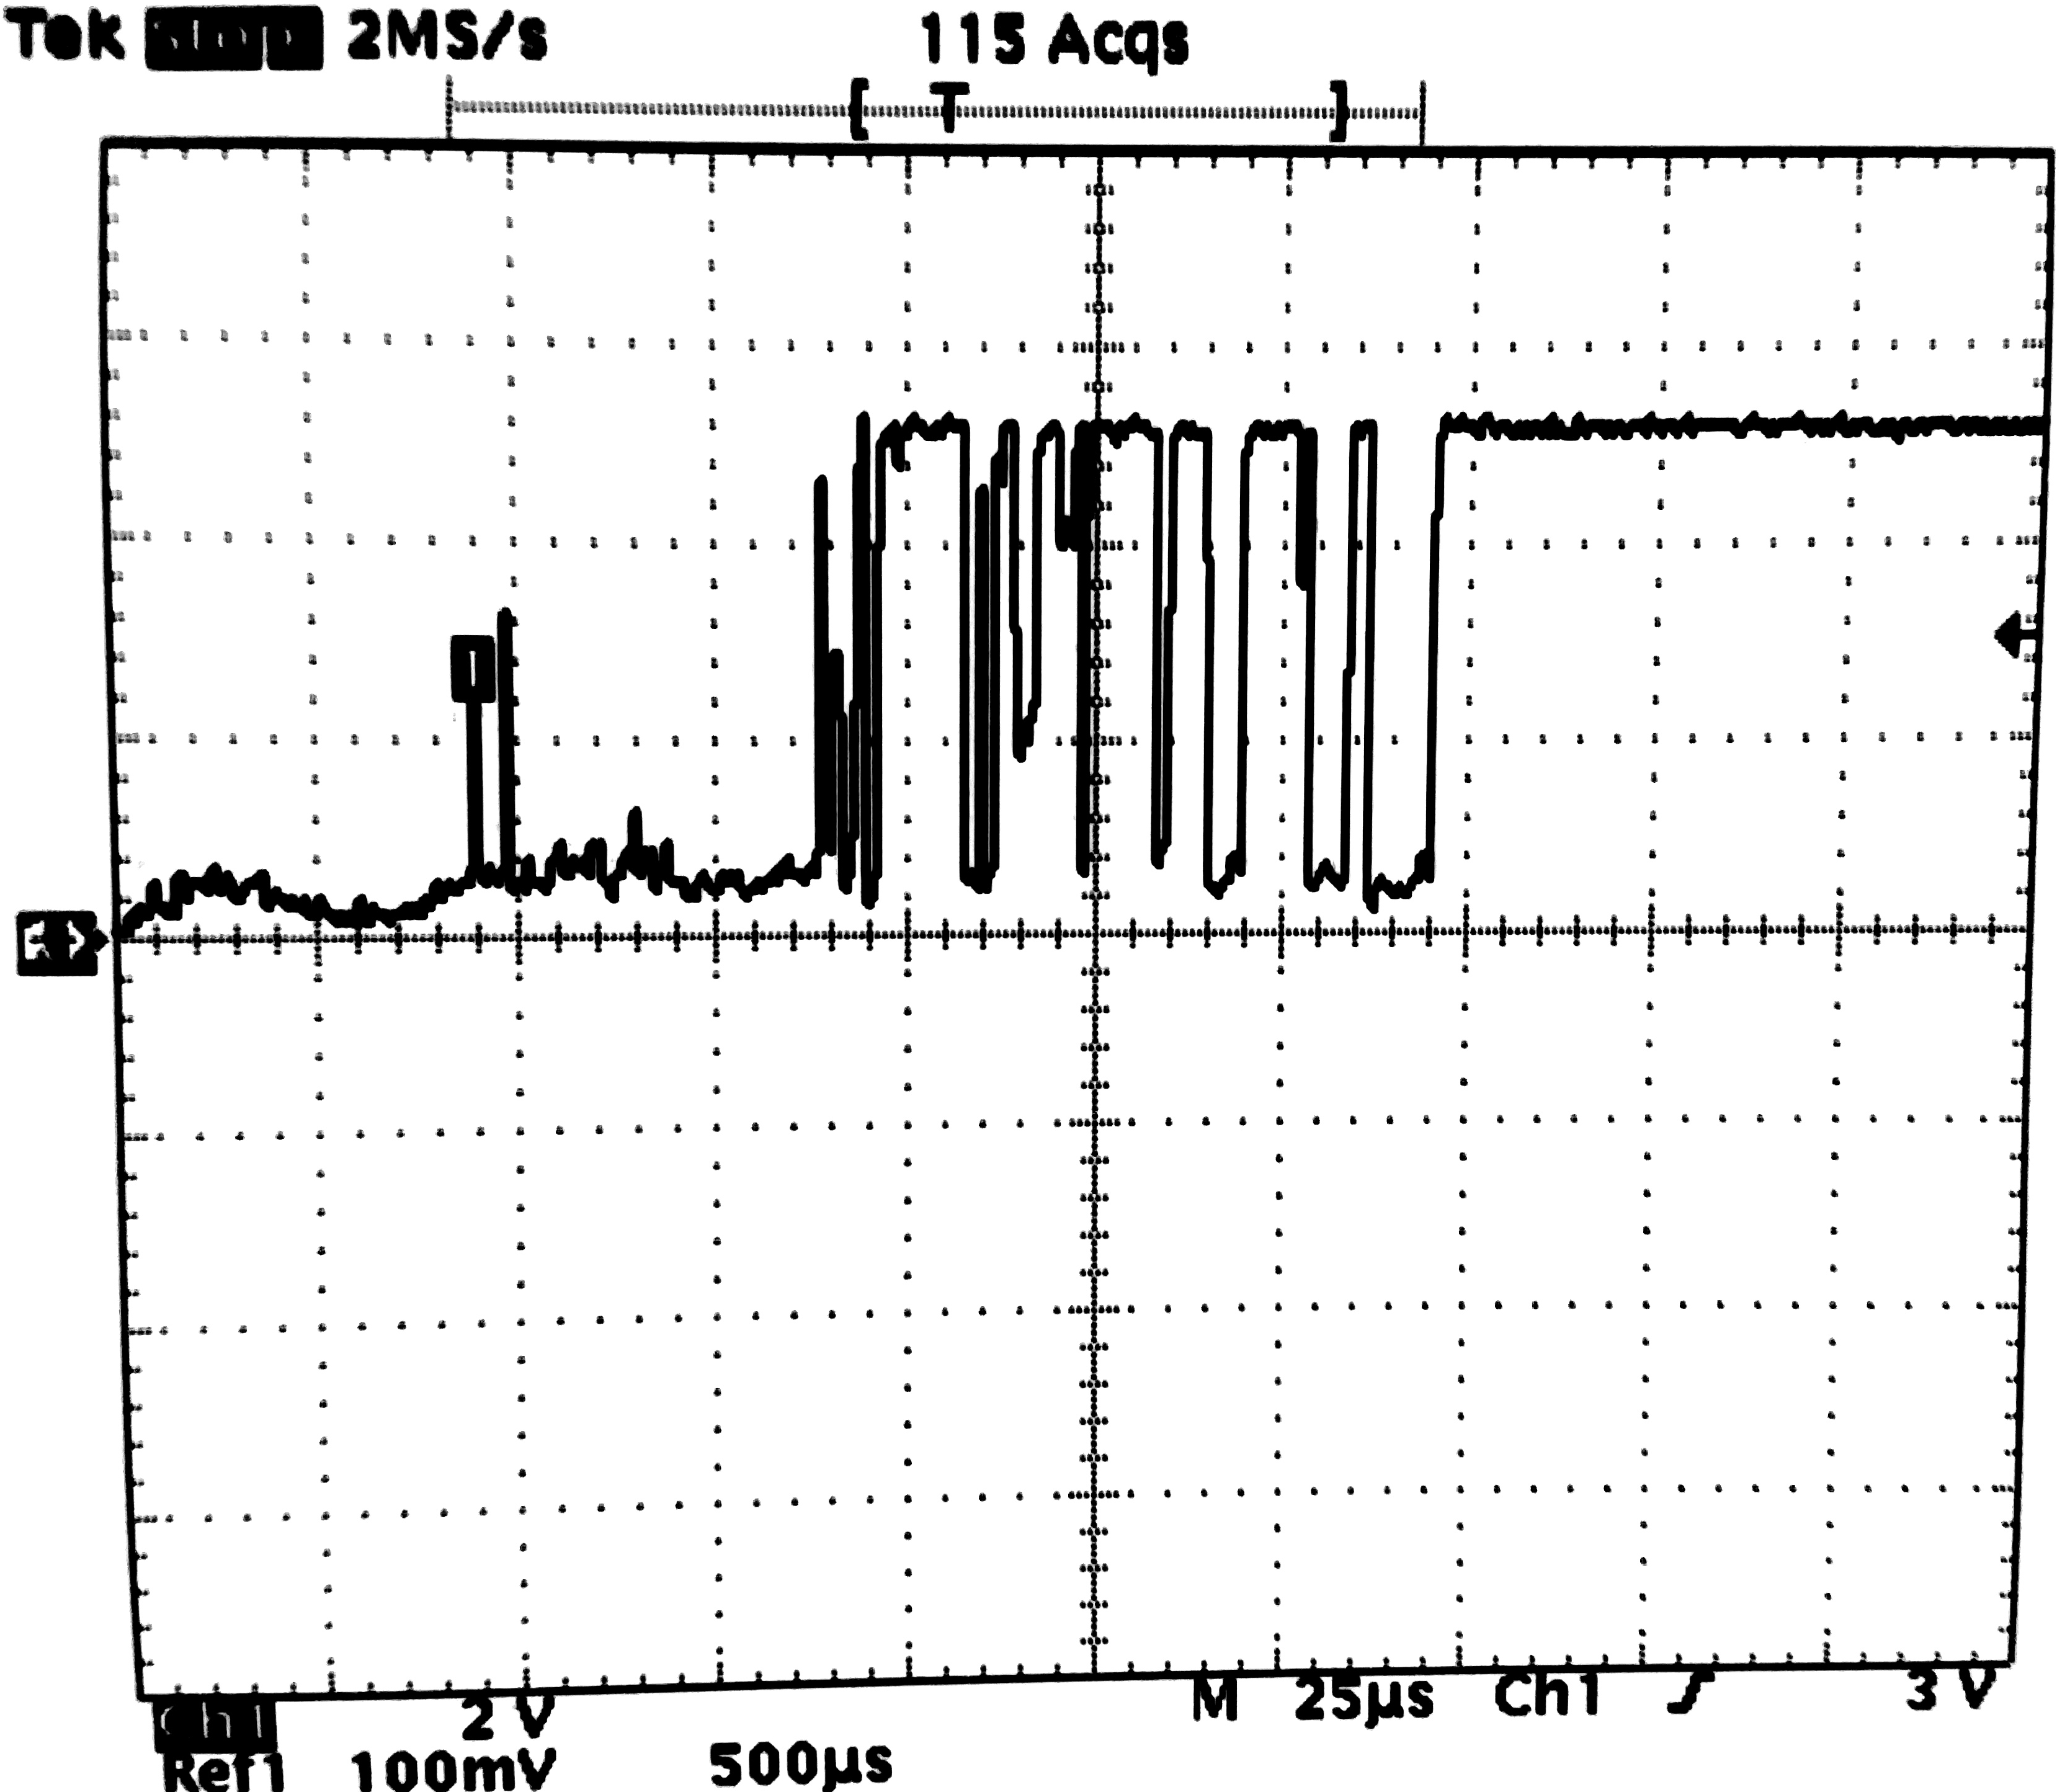
\includegraphics[scale=0.2]{debouncezao.png}
                    \caption{Ruído causado}
                    \label{fig:debounce2}
                \end{figure} \\
                
                \begin{figure}[H]
                    \centering
                    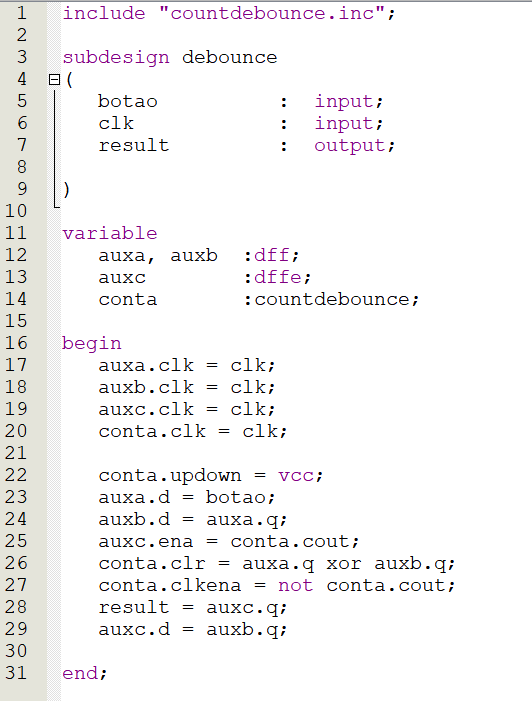
\includegraphics[scale=0.85]{modulo_debounce.PNG}
                    \caption{Módulo Debounce}
                    \label{fig:debounce}
                \end{figure} \\
                \tab Após a implementação do Debounce, o projeto foi testado em $3$ placas diferentes, de forma que funcionou de forma aceitável nas $3$ tendo como base o teste de pressionar rapidamente os botões.
                
            \section[Módulo Comparador]{\hyperlink{toc}{Módulo Comparador}}
                \tab O módulo Comparador foi idealizado para que pudesse ocorrer a comparação entre o horário atual e o horário definido para os despertadores, de forma que se ocorrer a igualdade e a chave de acionamento estiver ativada, quatro LEDs da placa são ativados em modo piscar durante o tempo de igualdade (os segundos são desconsiderados). \\
                \tab A lógica principal do comparador consiste em um \texit{case} cujas condições dependem das chaves acionadoras dos despertadores. \\
                
                
                \begin{figure}[H]
                    \centering                    
                    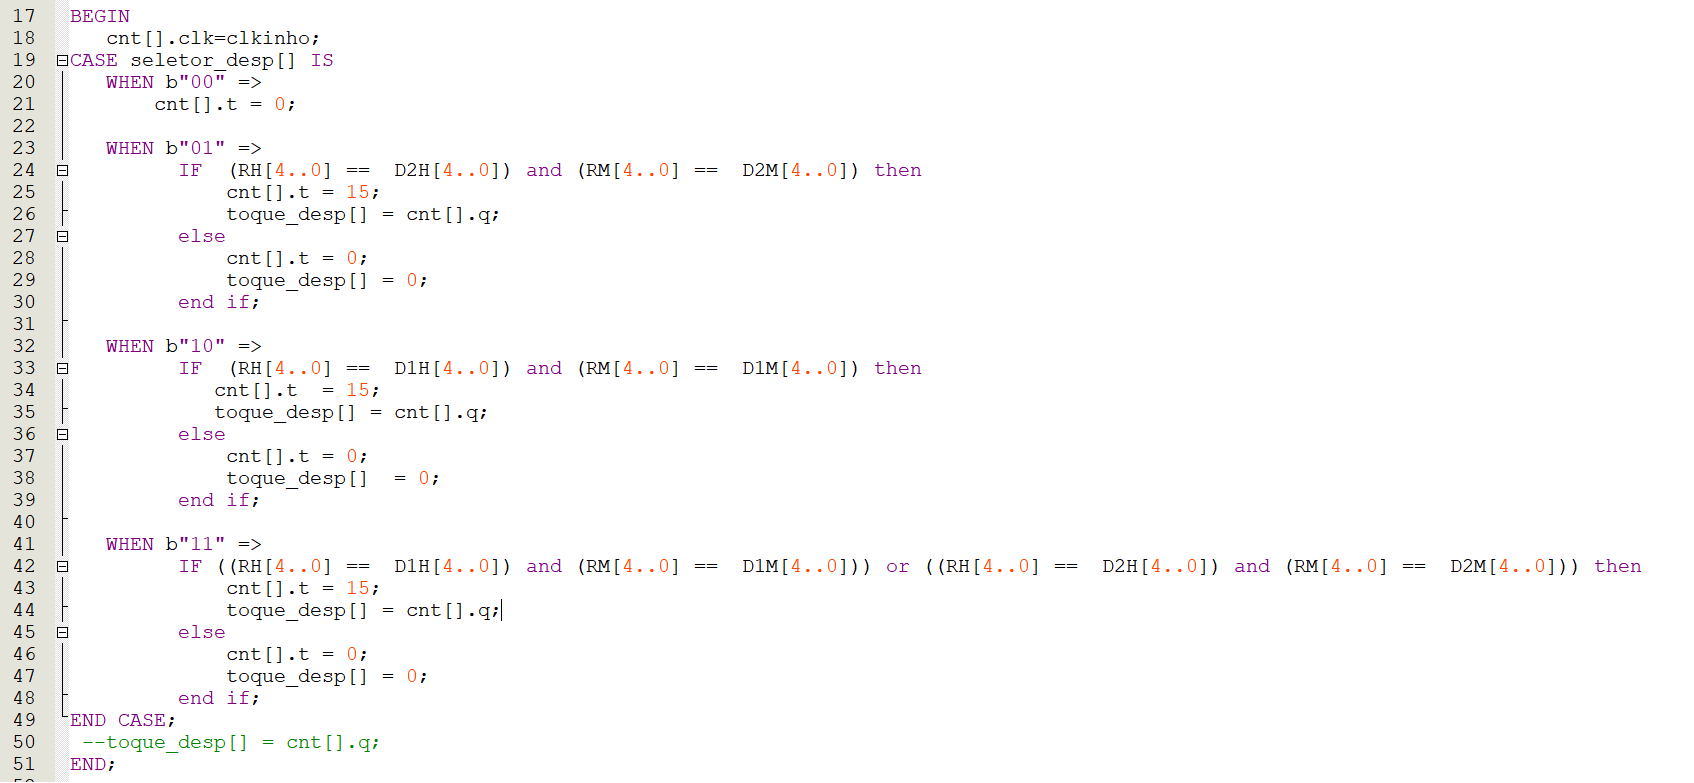
\includegraphics[scale = 0.62]{comparador.PNG}
                    \caption{Módulo Comparador}
                    \label{manual}
                \end{figure} \\
            \section[Módulo de Seleção de Operação]{\hyperlink{toc}{Módulo de Seleção de Operação}}
                \tab Como o projeto possui quatro modos de operação: Relógio, Despertadores e Cronômetro, foi preciso elaborar um módulo que pudesse estabelecer a relação de escolha do que seria mostrado nos displays de $7$ segmentos, por isso foi desenvolvido tal módulo, que envolve desde um mux para escolher entre o horário do relógio, despertadores ou cronômetro em bits (mux 4:1 de 5 ou 6 bits), um decodificador para transformar 5 ou 6 bits de informação em dois vetores de 4 bits de informação e um decodificador para ler o valor da informação de 4 bits em binário e passar para o display como números de base decimal. \\
                \begin{figure}[H]
                    \centering   
                    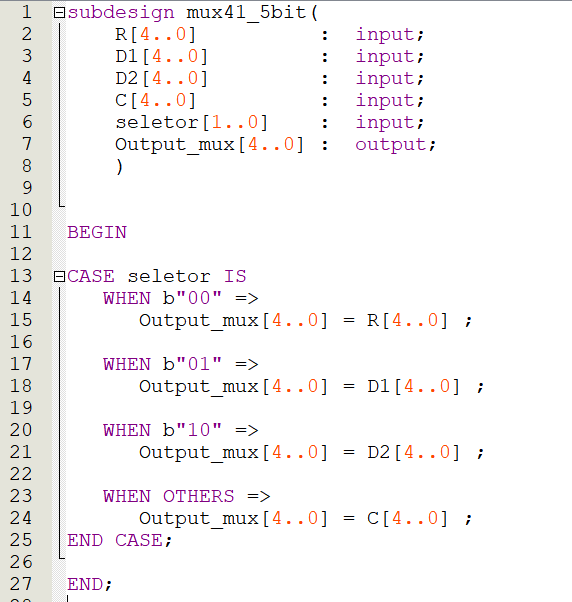
\includegraphics[scale = 1]{mux_41_5bit.PNG}
                    \caption{Mux 4:1 de cinco bits}
                    \label{mux41}
                \end{figure} \\
                \begin{figure}[H]
                    \centering                    
                    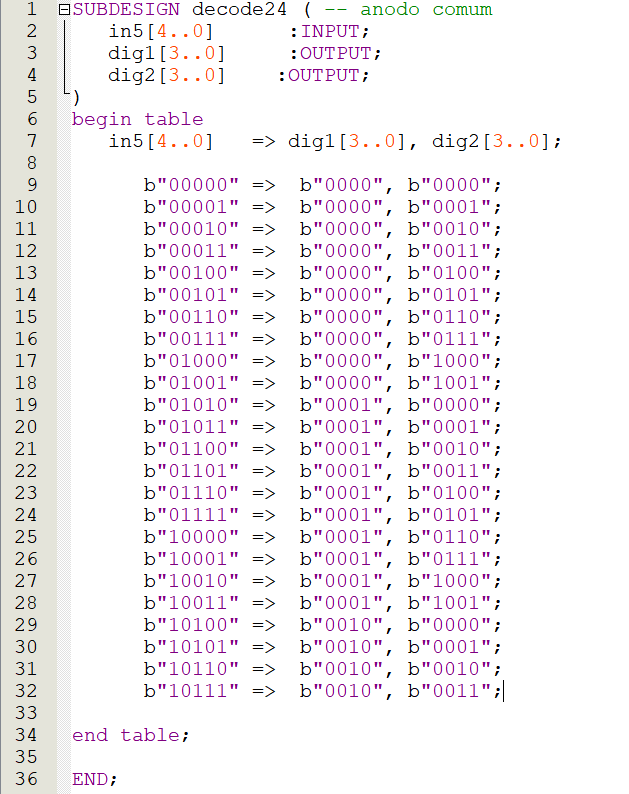
\includegraphics[scale = 1]{decode_5bit.PNG}
                    \caption{Decodificador de cinco bits}
                    \label{decodificador de 5 bits}
                \end{figure} \\
                \begin{figure}[H]
                    \centering                    
                    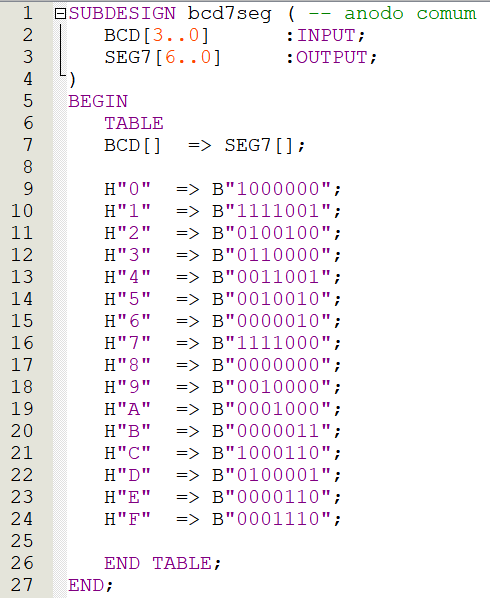
\includegraphics[scale = 1]{bcd_7seg.PNG}
                    \caption{Decodificador para o display de 7 segmentos}
                    \label{decodificador de 7 segmentos}
                \end{figure}
                
            \section[Módulo Indicador]{\hyperlink{toc}{Módulo Indicador}}    
                \tab Com o intuito de indicar o modo de operação que está exibido no displays de $7$ segmentos, foi implementado o Módulo que se aproveita de displays de $7$ segmentos não usador para horas, minutos ou segundos e usa os indicadores "H", "d1", "d2", ou "C" para apontar o modo de operação exibido. Sendo estes "horário", "despertador 1", "despertador 2", e "cronômetro" respectivamente.
                
                \tab O indicador possui como entradas as chaves seletoras \textbf{SW[16]} e \textbf{SW[15]}, que também são responsáveis por determinar o modo de operação exibido. 
                
                \tab A Figura \ref{indicador} mostra a implementação do Módulo Indicador
                
                    \begin{figure}[H]
                    \centering                    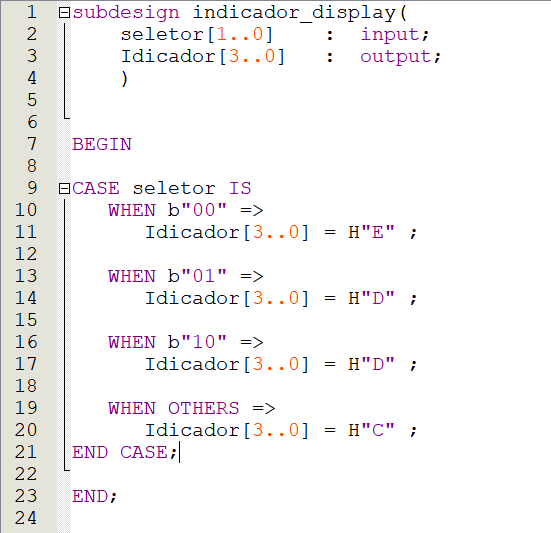
\includegraphics[scale = 0.9]{indicador_display.PNG}
                    \caption{Indicador de Operação}
                    \label{indicador}
                    \end{figure}
                Vale ressatar que a saída para o casa em que seletor $=$ "00" é igual a H"E". No entanto, observa-se que a tabela verdade do decodificador do display de $7$ segmentos foi alterada de forma que a saída correspondente a uma entrada H"E" seja mostrada como "H" no display.
                
                
                
         \chapter[Manual de Operação]{\hyperlink{toc}{Manual de Operação}}
                \tab Esta seção é dedicada a esclarecer o funcionamento e organização da placa da \textit{Altera DE2-115}, bem como explicitar quais chaves, displays, LEDs e botões foram utilizados na implementação do relógio, despertadores e cronômetro. \\
                \tab Observa-se um esquemático da placa na Figura \ref{manual}. Em que:
              
                    \begin{comment}\textbf{SW[17]} é a chave de ajuste ou exibição do que se encontra nos displays, \textbf{SW[16]} é a chave que determina a exibição do relógio ou despertador nos displays e \textbf{SW[15]} é a chave de acionamento do despertador, o LED da extrema direita é usado para indicar o modo de operação do despertador, enquanto o grupo de quatro LEDs indica igualdade entre despertador e relógio (toca alarme). Os quatro botões da placa são utilizados para realizar os incrementos e decrementos do relógio e despertador. O funcionamento desse botões são, respectivamente: incremento das horas, decremento das horas, incremento dos minutos e decremento dos minutos. \\
                    \end{comment}
                 \begin{itemize}
                \item \textbf{SW[17]} é a chave de ajuste ou exibição do relógio.
                
                \item \textbf{SW[16]} e \textbf{SW[15]} determinam, em conjunto, o que é exibido nos displays.
                
                \item \textbf{SW[14]} e \textbf{SW[13]} acionam os despertadores 1 e 2, respectivamente.
                
                \item \textbf{SW[3]} é a chave de ajuste ou exibição do despertador 1. 
                
                \item \textbf{SW[2]} é a chave de ajuste ou exibição do despertador 2.
                
                \item \textbf{SW[1]} é a chave de \textit{reset} do cronômetro.
                
                \item \textbf{SW[0]} é a chave de pausa do cronômetro.
                
                \item Os quatro botões da placa são utilizados para realizar os incrementos e decrementos do relógio e despertador. O funcionamento desse botões são, respectivamente: incremento das horas, decremento das horas, incremento dos minutos e decremento dos minutos.
                
                \item Os displays indicadores de exibição mostram "H", "d1", "d2" ou "C", para indicar o que está sendo exibido pelos restantes dos displays. 
                
            \end{itemize}
                
                \begin{figure}[H]
                    \centering                    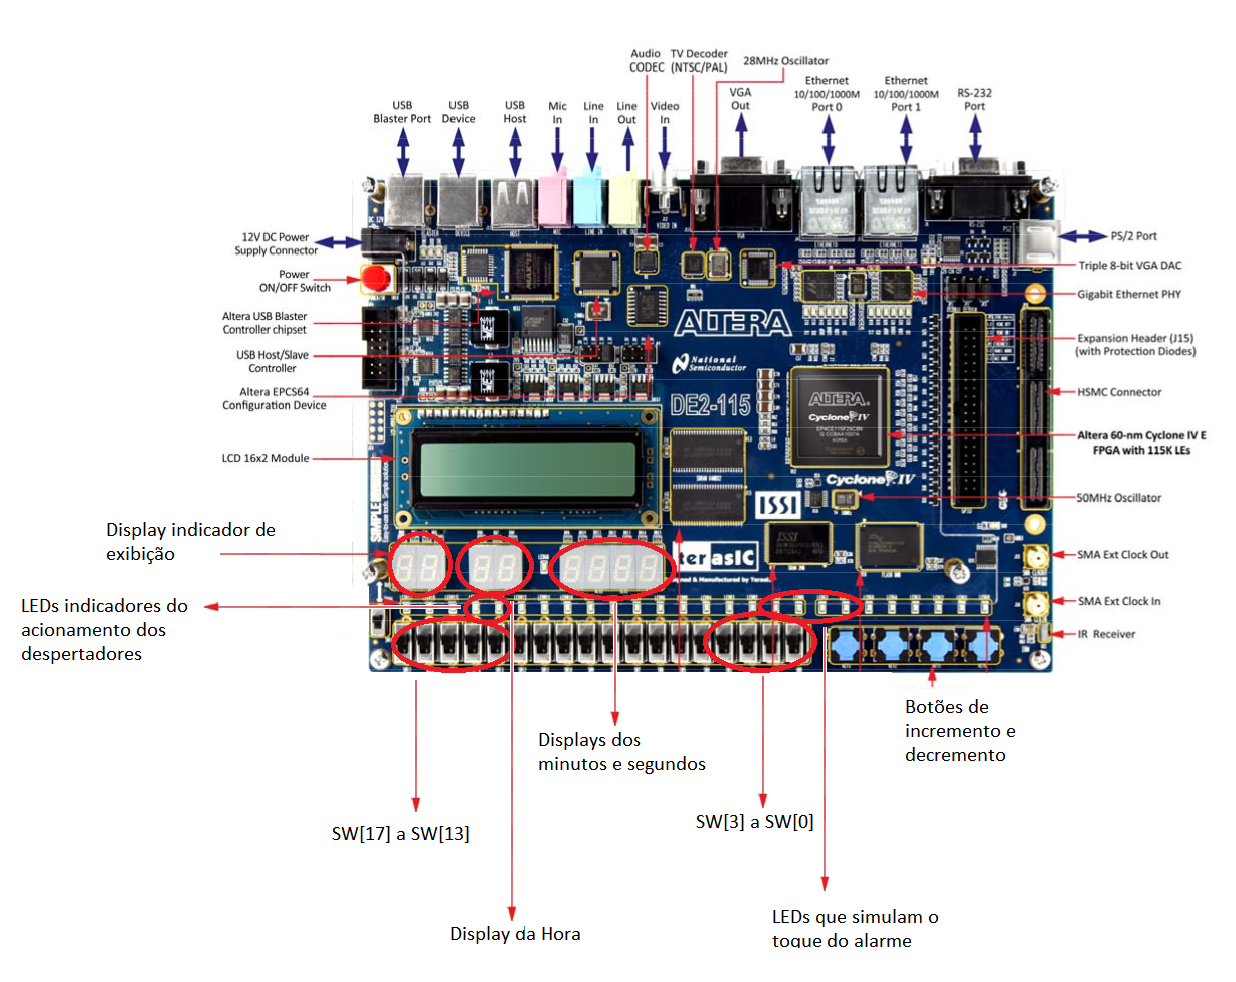
\includegraphics[width=\columnwidth]{manual_placa.png}
                    \caption{Manual de Operação}
                    \label{manual}
                \end{figure}
                
         
         \chapter[Resultados]{\hyperlink{toc}{Resultados}}
            
            \tab Observa-se a seguir a imagem do projeto final no \textit{Quartus}, o reultado obtido a partir da simulação do bloco do contador de módulo e fotos da placa operando nos diferentes modos de operação.
                
                \begin{figure}[H]
                    \centering
                    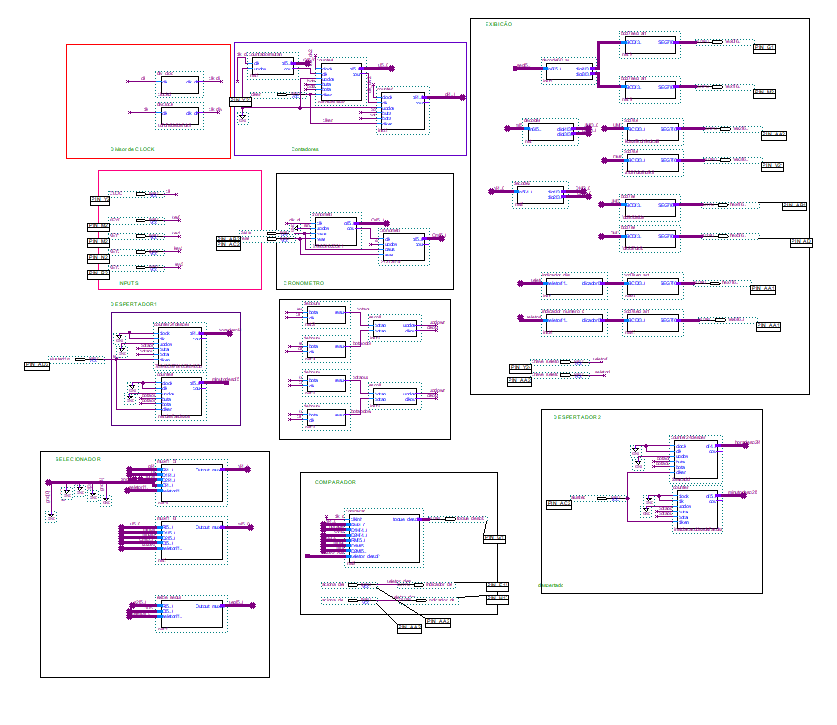
\includegraphics[width=\columnwidth]{projeto_final.PNG}
                    \caption{Projeto final}
                    \label{projeto final}
                \end{figure}
            
            
                \begin{figure}[H]
                    \centering
                    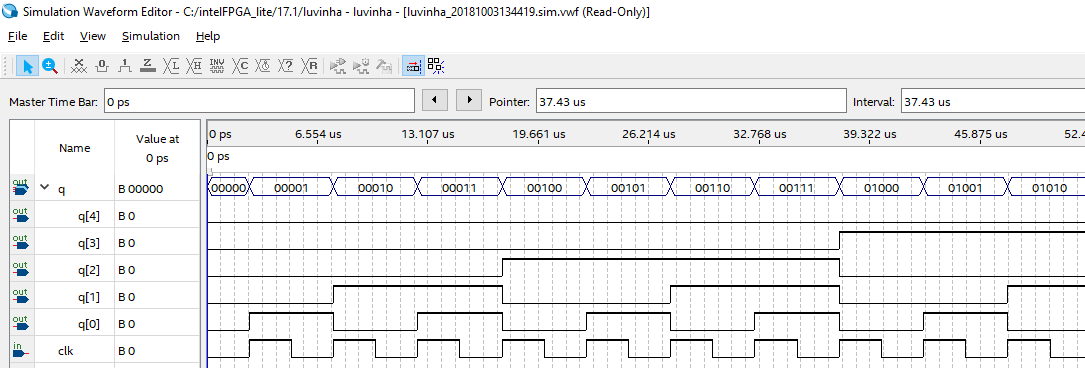
\includegraphics[width=\columnwidth]{simulacao_mod_24.png}
                    \caption{Simulação do bloco do contador de módulo 24}
                    \label{simulação_24}
                \end{figure}
                
                \begin{figure}[H]
                    \centering
                    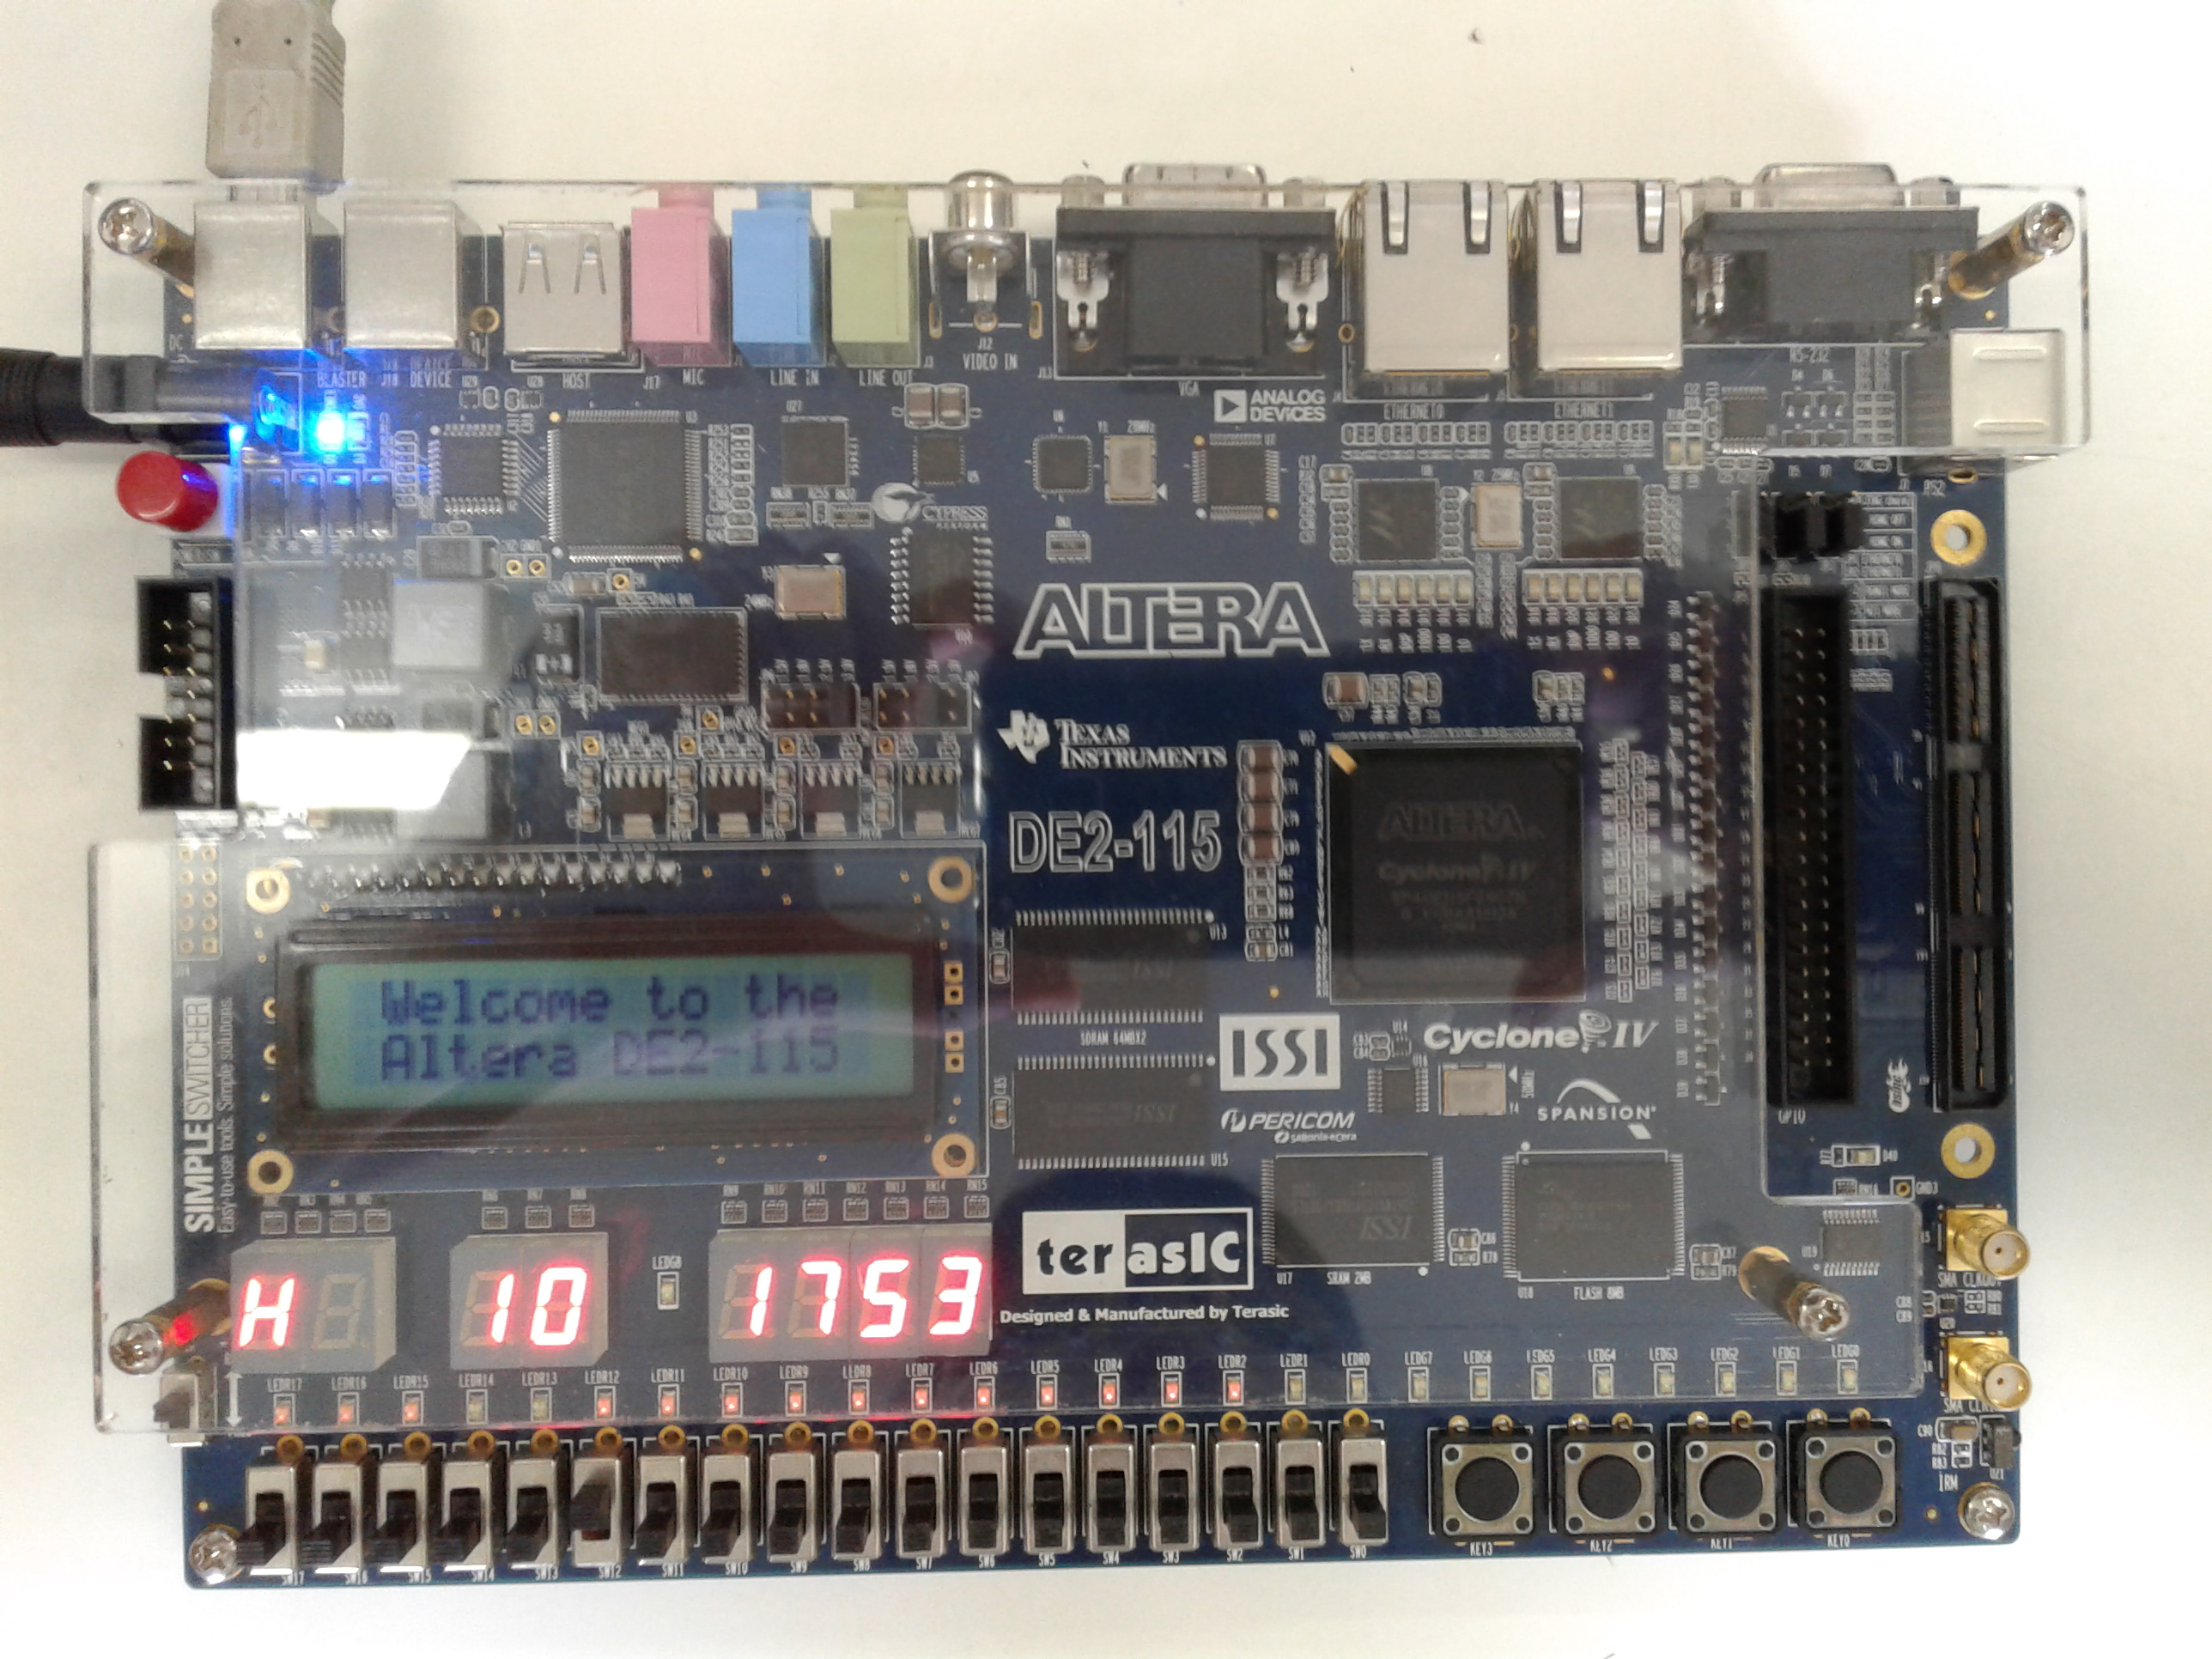
\includegraphics[width=\columnwidth]{foto_placa_H.jpg}
                    \caption{Foto da placa operando no modo horário (H)}
                    \label{foto_H}
                \end{figure}
                
               \begin{figure}[H]
                    \centering
                    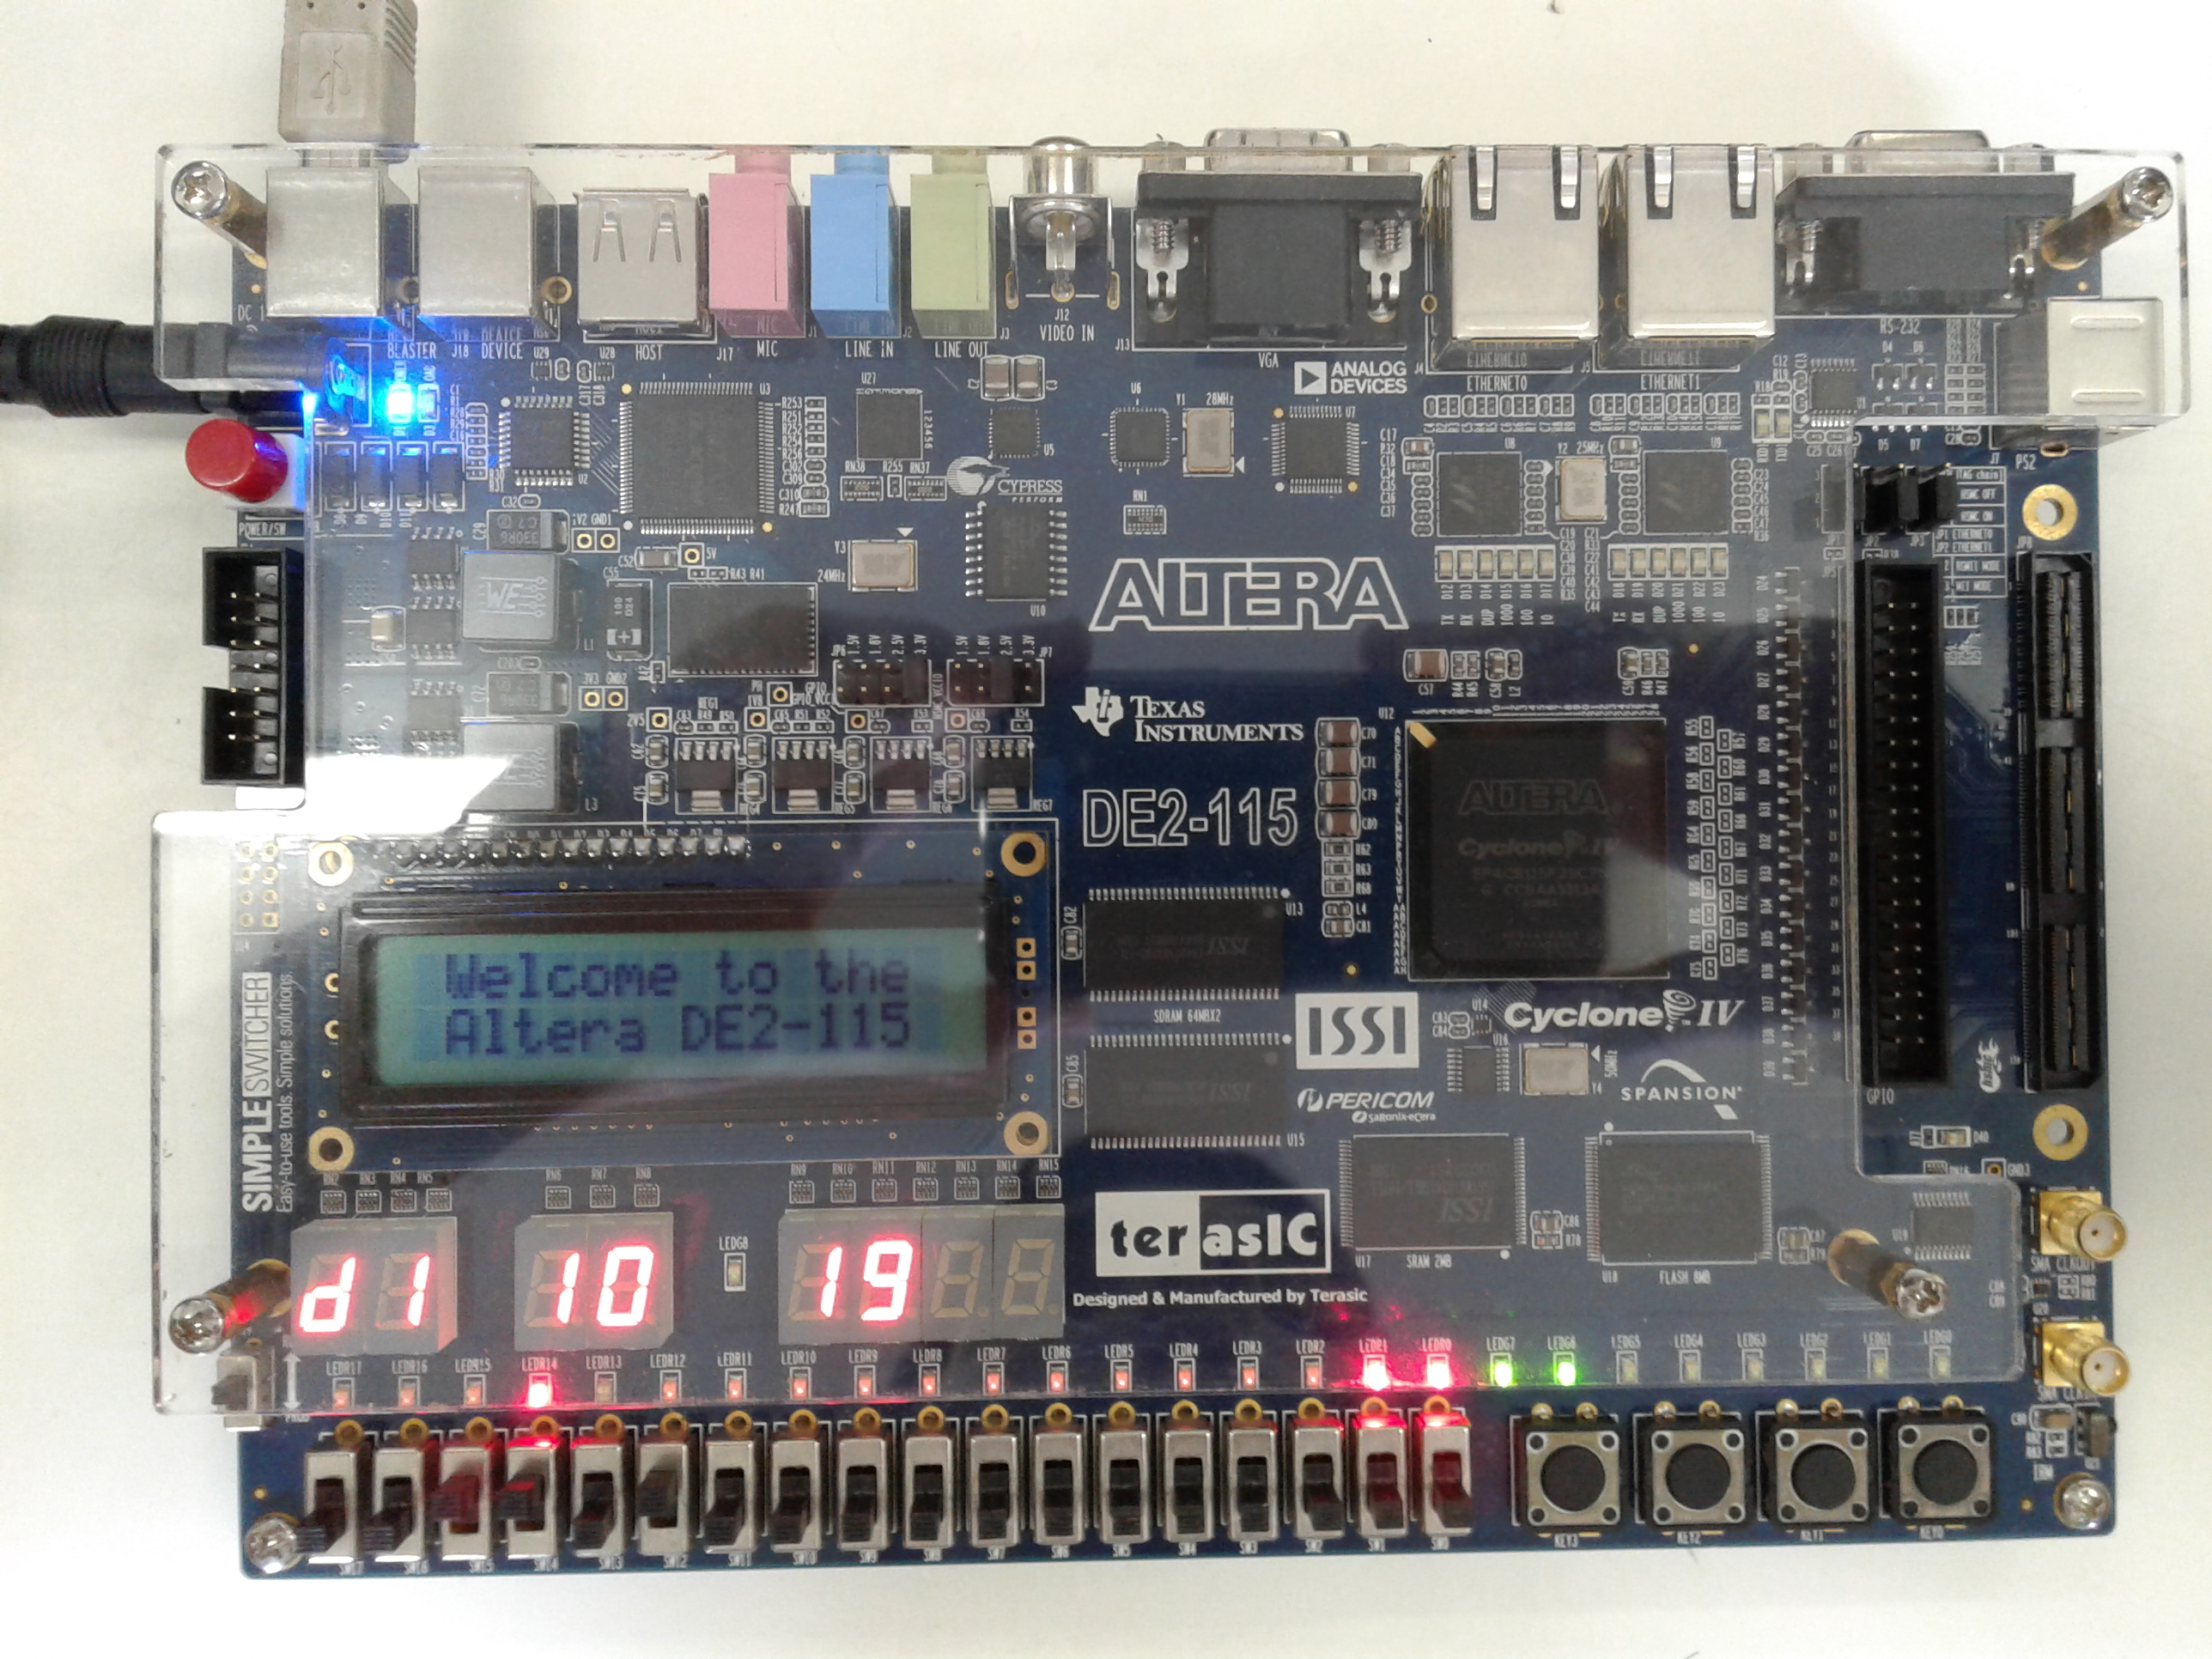
\includegraphics[width=\columnwidth]{foto_placa_d1.jpg}
                    \caption{Foto da placa operando no modo despertador 1 (d1)}
                    \label{foto_despertador1}
                \end{figure}
                
                \begin{figure}[H]
                    \centering
                    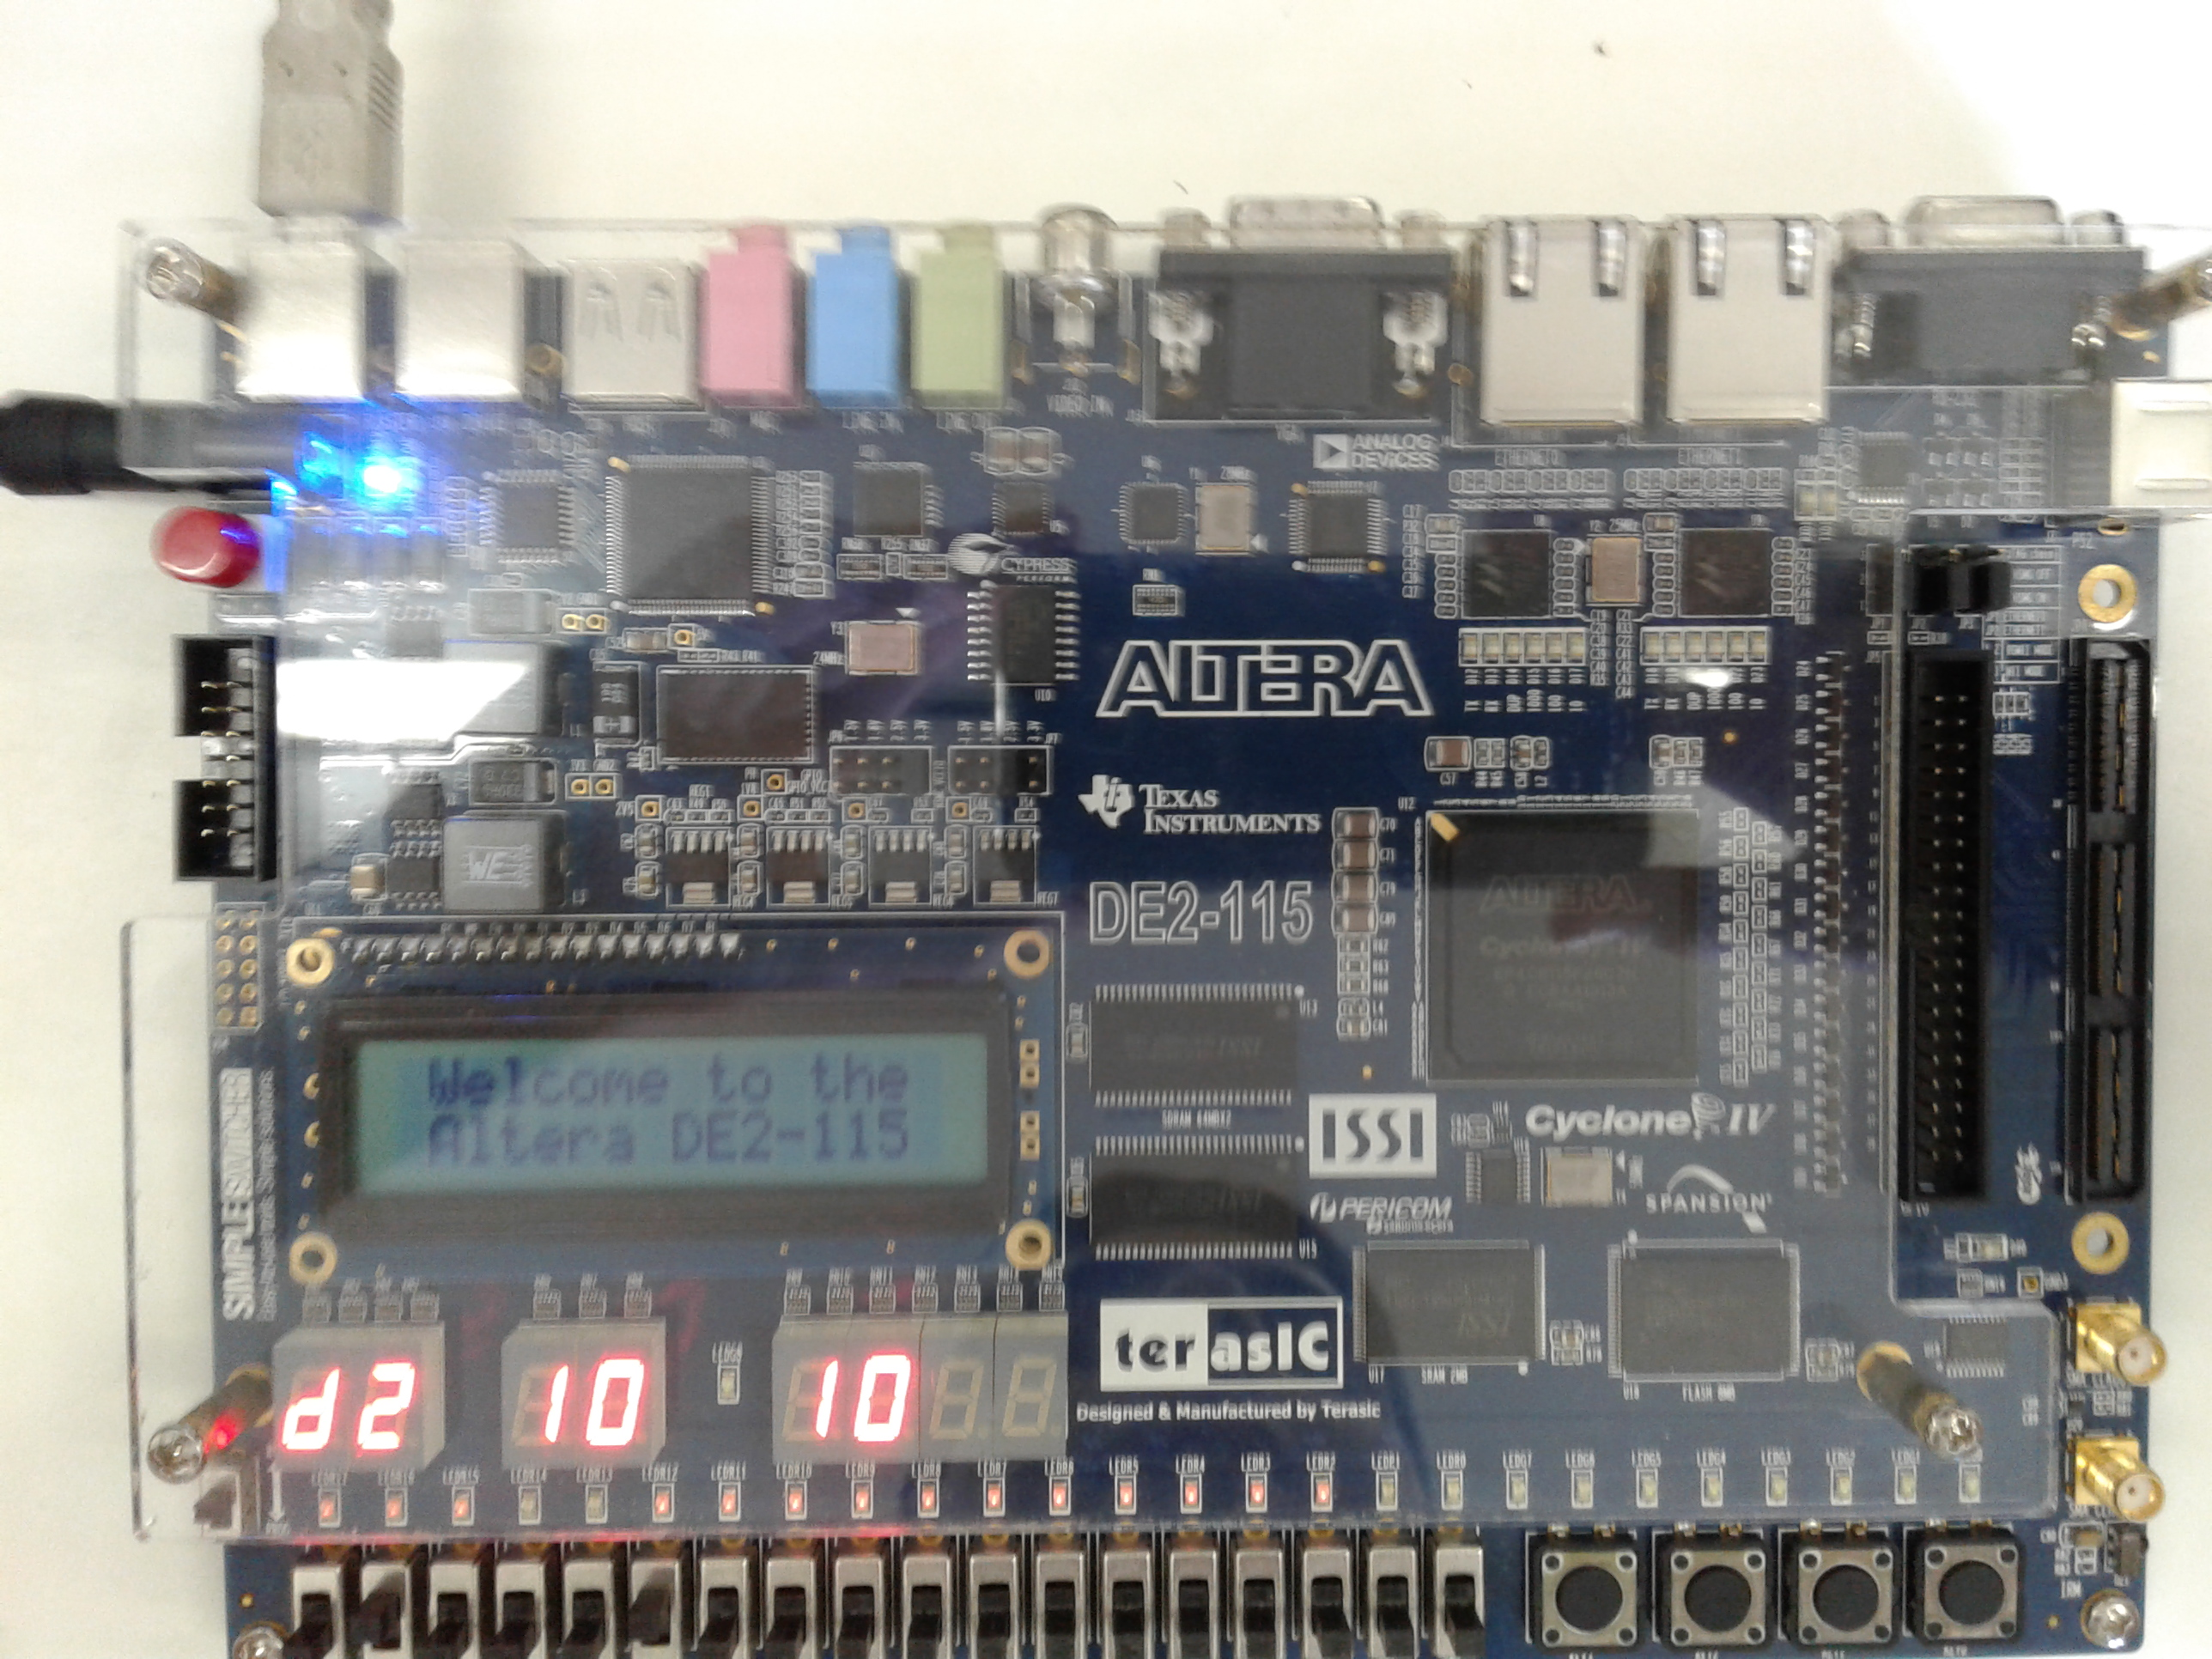
\includegraphics[width=\columnwidth]{foto_placa_d2.jpg}
                    \caption{Foto da placa operando no modo despertador 2 (d2)}
                    \label{foto_despertador2}
                \end{figure}
                
                \begin{figure}[H]
                    \centering
                    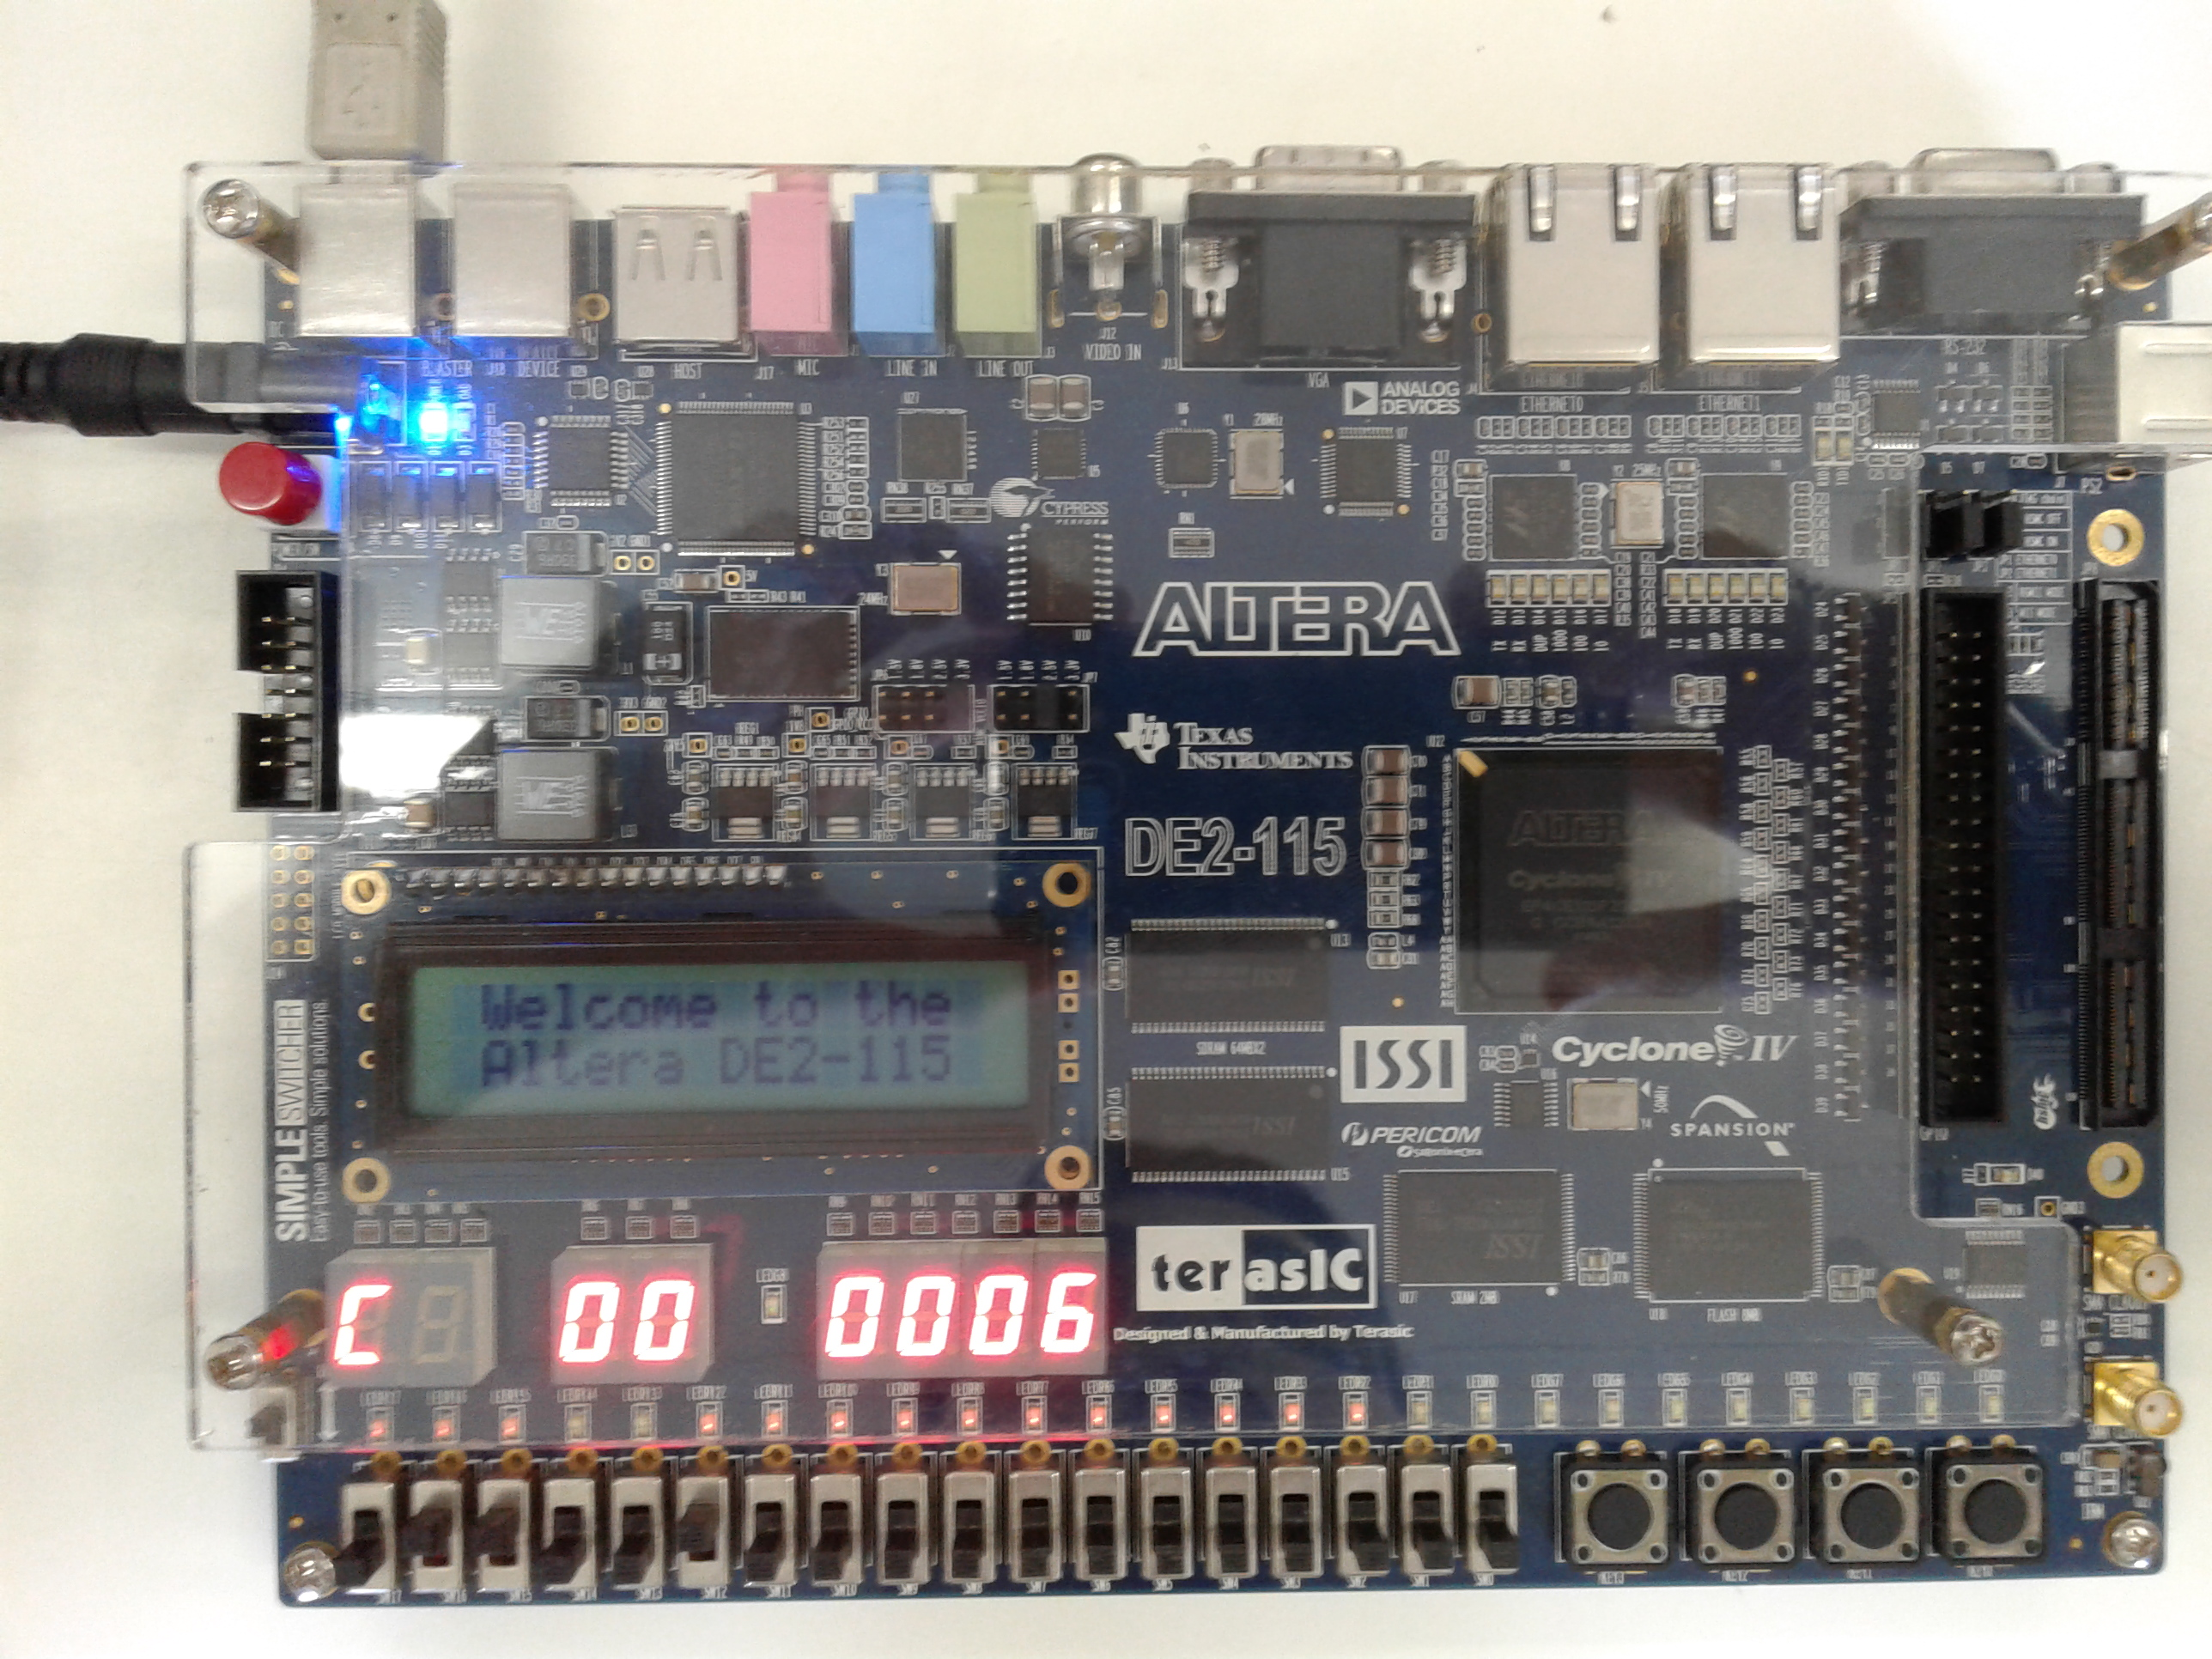
\includegraphics[width=\columnwidth]{foto_placa_C.jpg}
                    \caption{Foto da placa operando no modo cronômetro (C)}
                    \label{foto_cronometro}
                \end{figure}
         
         
         
         
            
        \chapter[Discussão]{\hyperlink{toc}{Discussão}} \hypertarget{ana}{}
            \tab No tocante aos problemas e dificudades encontrados no desenvolvimento do projeto cita-se a implementação do cronômetro com a função reset independente da função \textit{pause}, além da adaptação do projeto as especificações da placa.
            \section[Cronômetro]{\hyperlink{toc}{Cronômetro}}
                
                 \tab No cronômetro, foi decidido pelo grupo que não seria interessante mostrar no display o valor da hora. Portanto, na passagem pelo decodificador, foi imposto os valores $0$ sobre a hora.
                
                \tab Nota-se também que não conseguimos executar a função de \textit{reset} de maneira perfeita a nao ser que executado em conjunto com a função \textit{pause}, da mesma forma que cronômetros comerciais, o que não trouxe grandes impactos ao funcionamento do relógio e do cronômetro em si, logo preferimos manter o funcionamento atual. Quanto as especificações da placa tivemos que lidar com o fato do botoes serem ativos em baixo , vide Figura \ref{fig:cronometro}. \\
                
                
            \section[Botões]{\hyperlink{toc}{Botões}}
                \tab  Mediante as especificações da placa tivemos que lidar com o fato dos botões serem ativos em baixo ou seja, ao serem pressionados, o sinal teria nível lógico zero, um tanto quanto diferente do esperado porém facilmente solucionável, além disso os botões possuem um sistema de debounce contendo um disparador Schmitt Trigger que se mostrou não muito confiável, então implementamos um sistema de debounce auxiliar para garantir o bom funcionamento dos botões, esse debounce também foi acrescido de um sistema de escolha onde o próprio botão indica qual será o processo seja de incremento e decremento o sistema de debounce implementado juntamente com o sistema de escolha, vide Figura \ref{fig:debounce2}. \\
                
                
                \begin{figure}[H]
                    \centering
                    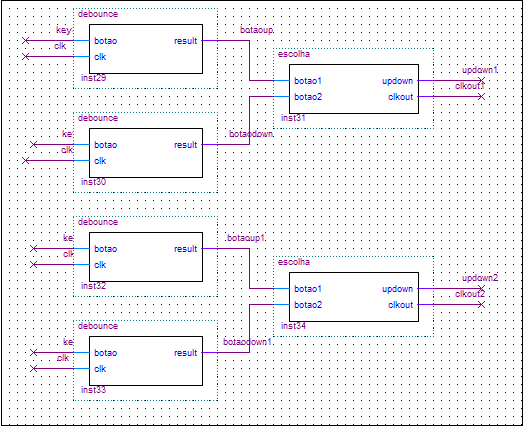
\includegraphics[scale=0.7]{debounce2.png}
                    \caption{Debounce e Escolha}
                    \label{fig:debounce2}
                \end{figure} \\
                
                
            \section[Chaves]{\hyperlink{toc}{Chaves}}
                \tab Ainda devido as especificações da placa temos a questão das chaves, diferentemente dos botões as chaves não possuem um debounce incluso na placa, devido ao fato de seu estado ser mais fácil de definir e estabilizar mecanicamente, pois trava nas posições de nível lógico alto e baixo, chave para cima e para baixo respectivamente, diante disto e do fato de não trazer grandes distúrbios quando usada não aplicamos o modulo debounce às chaves usadas.\\
            \section[\textit{Display}]{\hyperlink{toc}{\textit{Display}}}
                \tab como ultima especificação temos o \textit{display} de $7$ segmentos, o \textit{display} da placa é ativo no nivel logico baixo, catodo comun, sendo preciso levar isto em conta na implementaçao do código. Cada \textit{display} possuí tambem um numero limitado de LEDs sendo estes $7$ que sen encontram distribuídos em formato de número $8$ e um ponto decimal, fato este que limita a possibilidade de números e letras que podem ser representados.\\
                
            \section[Contador]{\hyperlink{toc}{Contador}}
                \tab Diferentemente do projeto em código de blocos o desenvolvimento do contador não apresentou grandes problemas, foram feitos 3 blocos um para o contador de segundos, outro para o de minutos, ambos com modulo 60 e um modulo 24 para as horas, primeiro foi pensado em implementar um contador onde os botões agissem diretamente no \textit{clock} dos blocos contadores, porém devido a problemas de armazenamento de dados e de interatividade com os comandos de incremento dos botões decidimos por um modelo em que o botão não atua no \textit{clock} e sim como um processo de incremento a parte, o contador está ilustrado na Figura \ref{bloco contador}. \\
                \begin{figure}[H]
                    \centering
                    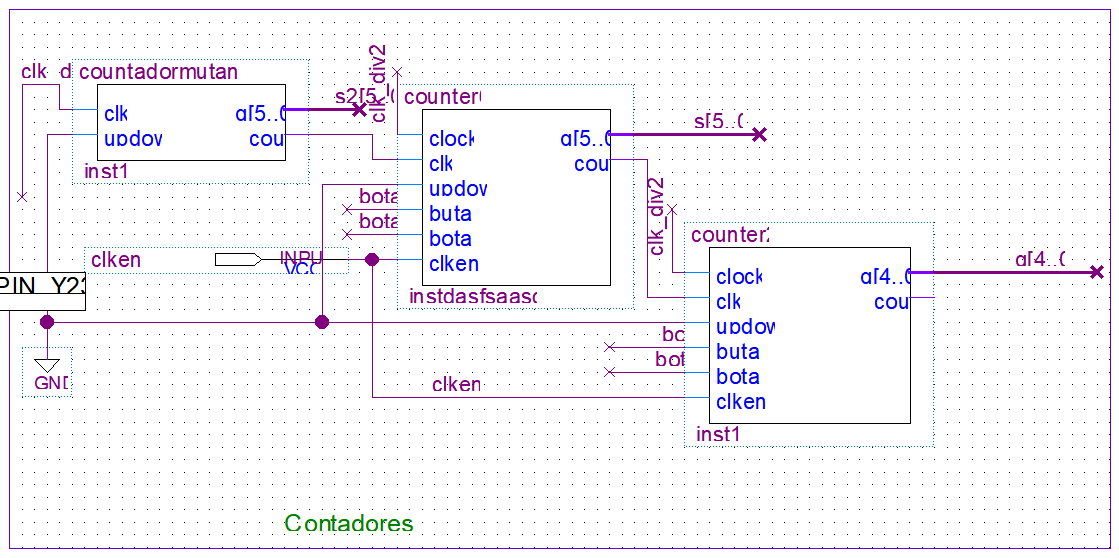
\includegraphics[scale=0.7]{bloco_contador.PNG}
                    \caption{Bloco dos Contadores do Relógio}
                    \label{bloco contador}
                \end{figure} \\
                
        \chapter[Conclusão]{\hyperlink{toc}{Conclusão}}
            \tab Observa-se que o relógio e o cronômetro operam em contagem crescente de forma síncrona e esperada. Ao incrementar ou decrementar alguma das funções do projeto, nota-se a consistência do que foi feito e que, até o presente momento, bugs e limitações não foram detectados. Também é digno de nota que, problemas encontrados no projeto anterior, referentes a incrementação e decrementação, foram resolvidos neste projeto sem maiores transtornos. \\
            \tab Ao contrário do que foi argumentado nesta mesma seção no projeto anterior, desta vez, a implementação das especificações foi bem simples, visto que usamos estruturas condicionais e mudamos o modelo de contador, agora sendo uma calculadora movida a pulsos de clock. Sendo assim, é fácil notar que, para projetos em que circuitos já são visualizados ou já estão planejados, a linguagem AHDL se torna uma grande ferramenta que simplifica e agiliza o processo de implementação deste circuito.
                    
        
        
\end{document}